%%%%%%%%%%%%%%%%%%%%%%%%%%%%%%%%%%%%%%%%%%%%%%%%%%%%%%%%%%%%%%%%%%%%%
%
%  This is a sample LaTeX input file for your contribution to 
%  the MC2013 conference. Modified by R.C. Martineau at INL from A. 
%  Sood at LANL, from J. Wagner ORNL who obtained the original class 
%  file by Jim Warsa, LANL, 16 July 2002}
%
%  Please use it as a template for your full paper 
%    Accompanying/related file(s) include: 
%       1. Document class/format file: mc2013.cls
%       2. Sample Postscript Figure:   figure.eps
%       3. A PDF file showing the desired appearance: template.pdf 
%    Direct questions about these files to: richard.martinea@inl.gov
%
%    Notes: 
%      (1) You can use the "dvips" utility to convert .dvi 
%          files to PostScript.  Then, use either Acrobat 
%          Distiller or "ps2pdf" to convert to PDF format. 
%      (2) Different versions of LaTeX have been observed to 
%          shift the page down, causing improper margins.
%          If this occurs, adjust the "topmargin" value in the
%          mc2013.cls file to achieve the proper margins. 
%
%%%%%%%%%%%%%%%%%%%%%%%%%%%%%%%%%%%%%%%%%%%%%%%%%%%%%%%%%%%%%%%%%%%%%


%%%%%%%%%%%%%%%%%%%%%%%%%%%%%%%%%%%%%%%%%%%%%%%%%%%%%%%%%%%%%%%%%%%%%
\documentclass{mc2013}
%
%  various packages that you may wish to activate for usage 
\usepackage{graphicx}
\usepackage{tabls}
\usepackage{afterpage}
\usepackage{cites}
\usepackage{amssymb}
\usepackage{amsfonts}
\usepackage{amsmath}
\usepackage{amsthm}
\usepackage[mathcal]{euscript}
\usepackage{tmadd,tmath}

%\usepackage{epsf}
%
%
% Insert authors' names and short version of title in lines below
%
\newcommand{\authorHead}      % Author's names here
   {Slattery, Wilson, and Evans}  
\newcommand{\shortTitle}      % Short title here
   {Domain Decomposed Neumann-Ulam Method}  
%%%%%%%%%%%%%%%%%%%%%%%%%%%%%%%%%%%%%%%%%%%%%%%%%%%%%%%%%%%%%%%%%%%%%
%
%   BEGIN DOCUMENT
%
%%%%%%%%%%%%%%%%%%%%%%%%%%%%%%%%%%%%%%%%%%%%%%%%%%%%%%%%%%%%%%%%%%%%%
\begin{document}

%
%      Headers and Footers
\afterpage{%
\fancyhf{}%
\fancyhead[CE]{              
{\scriptsize \authorHead}}                                                
\fancyhead[CO]{               
{\scriptsize \shortTitle}}                  
%\lfoot{\scriptsize{
%International Conference on Mathematics and Computational Methods
%Applied to Nuclear Science \& Engineering (M\&C 2013), 
%\\ Sun Valley, Idaho, USA, May 5-9, 2013.}}%
\rfoot{\thepage/\totalpages{}}%

\pagestyle{fancy}
%\setlength{\topmargin}{-20pt}
}
 
\normalsize

\setlength{\baselineskip}{16.8pt}
\vspace{-3pt}

% 
% TITLE
%

\begin{center}
\textbf{\large \\% 
A SPECTRAL ANALYSIS OF THE DOMAIN DECOMPOSED ADJOINT MONTE CARLO
METHOD FOR LINEAR OPERATOR EQUATIONS}
% 
% First AUTHORS 
%
\\
\setlength{\baselineskip}{14pt}
\textbf{S.R. Slattery and P.P.H. Wilson} \\
Engineering Physics Department \\
University of Wisconsin - Madison  \\
1500 Engineering Dr., Madison, WI 53706 \\
sslattery@wisc.edu; wilsonp@engr.wisc.edu \\

% 
% SECOND AUTHORS (if not needed delete from here) 
%
\vspace{12pt}
\textbf{T.M. Evans} \\
Oak Ridge National Laboratory \\
1 Bethel Valley Road, Oak Ridge, TN 37830 \\
evanstm@ornl.gov \\ 
%
% SECOND AUTHORS (to here)
%

\end{center}

%
% SET RAGGED RIGHT MARGIN
%
\raggedright


\section*{ABSTRACT} 
\begin{quote}
\begin{small}
The domain decomposed behavior of the adjoint Neumann-Ulam Monte Carlo
method for solving linear operator equations is analyzed using the
spectral properties of the linear operator. Relationships for the
average length of the adjoint random walks, a measure of convergence
speed and serial performance, are made with respect to the Eigenvalues
and other properties of the linear operator. In addition,
relationships for the effective optical thickness of a domain in the
decomposition are presented based on the spectral analysis and
diffusion theory. Using the effective optical thickness, the Wigner
rational approximation and the mean chord approximation are applied to
estimate the leakage fraction of stochastic histories from a domain in
the decomposition as a measure of parallel performance and potential
communication costs. The one-speed, two-dimensional neutron diffusion
equation is used as a model problem to test the models for symmetric
operators. In general, the derived approximations show good agreement
with measured computational results.

\emph{Key Words}: Monte Carlo domain decomposition MCSA
\end{small} 
\end{quote}

\setlength{\baselineskip}{14pt}
\normalsize

%%---------------------------------------------------------------------------%%
\Section{INTRODUCTION}
\label{sec:intro}

An alternative approach to approximate matrix inversion is to employ
Monte Carlo methods that sample a distribution with an expectation
value equivalent to that of the inverted operator. Such methods have
been in existence for decades with the earliest reference noted here
an enjoyable manuscript published in 1950 by Forsythe and Leibler
\cite{forsythe_matrix_1950}. In their outline, Forsythe and Liebler in
fact credit the creation of this technique to J. Von Neumann and
S.M. Ulam some years earlier than its publication. In 1952 Wasow
provided a more formal explanation of Von Neumann and Ulam's method
\cite{wasow_note_1952} and Hammersley and Handscomb's 1964 monograph
\cite{hammersley_monte_1964} and Spanier and Gelbard's 1969 book
\cite{spanier_monte_1969} present additional detail on a method
adjoint to that described by Neumann and Ulam. In recent years, the
adjoint Neuman-Ulam method has been leveraged in Monte Carlo Synthetic
Acceleration (MCSA) methods that are competitive with conventional
methods including Krylov methods and are applicable to a wide variety
of linear systems \cite{evans_monte_2009,evans_monte_2012}. To advance
the applicability of these new MCSA methods, we therefore aim to apply
the underlying Monte Carlo methods to large-scale problems in parallel
computing environments.

To enable higher fidelity reactor physics Monte Carlo simulations,
domain decomposition has been identified as a key principle in moving
forward in high performance computing
\cite{brunner_comparison_2006,siegel_analysis_2012}. To accomplish
this, we recognize from the literature that stochastic histories must
be transported from domain to domain as the simulation progresses and
they transition to states that are not in the local domain. Because we
have chosen a domain decomposition strategy in a parallel environment,
this means that communication of these histories must occur between
compute nodes owning neighboring pieces of the global domain. We wish
to characterize this communication not only because communication is
in general expensive, but also because these nearest-neighbor
communication sequences have poor algorithmic strong scaling
\cite{gropp_high-performance_2001}.

The purpose of this study is to provide a simple, analytic theory
based on the properties of the linear system the will allow for
estimates of the domain decomposed behavior of the adjoint
Neumann-Ulam method. When solving problems where the linear operator
is symmetric, a host of analytic theories exist based on the
Eigenvalue spectrum of the operator that characterize their behavior
in the context of deterministic linear solvers. Using past work, these
theories are adapted to the domain decomposed adjoint Neumann-Ulam
method using the one-speed, two-dimensional neutron diffusion
equation. In this paper we describe the adjoint Neumann-Ulam Monte
Carlo method followed by a presentation of the model problem. Using
the linear system generated by this discretization, we use a spectral
theory to generate analytic relations for the Eigenvalues of the
operator based on system parameters. Using the Eigenvalue spectra, we
then build relationships to characterize the transport of stochastic
histories in a decomposed domain and the fraction of histories that
leak from a domain and will therefore have to be
communicated. Finally, we compare these analytic results to numerical
experiments conducted with the model problem and draw conclusions
looking towards future work.

%%---------------------------------------------------------------------------%%
\Section{ADJOINT NEUMANN-ULAM METHOD} 
\label{sec:adjoint_nu}

We seek solutions of the general linear problem in the following form:
\begin{equation}
  \ve{A} \ve{x} = \ve{b}\:.
  \label{eq:linear_problem}
\end{equation}
Choosing the adjoint method Monte Carlo method to invert the linear
operator, we define the linear system adjoint to
Eq~(\ref{eq:linear_problem}):
\begin{equation}
  \ve{A}^T \ve{y} = \ve{d}\:,
  \label{eq:adjoint_linear_problem}
\end{equation}
where $\ve{y}$ and $\ve{d}$ are the adjoint solution and source
respectively and $\ve{A}^T$ is the adjoint operator. We can derive a
Monte Carlo estimator from the adjoint method that will also give the
solution vector, $\ve{x}$. We first rearrange
Eq~(\ref{eq:adjoint_linear_problem}) as:
\begin{equation}
  \ve{y} = (\ve{I} - \ve{H}^T)^{-1} \ve{d}\:,
  \label{eq:adjoint_split_system_2}
\end{equation}
where $\ve{H} = \ve{I} - \ve{A}$ is the \textit{iteration matrix}.
This yields the adjoint Neumann series:
\begin{equation}
  \ve{y} = \sum_{k=0}^{\infty} (\ve{H}^T)^k\ve{d}\:.
  \label{eq:adjoint_neumann_series}
\end{equation}
For this series to converge, we require that the spectral radius of
$\ve{H}$ must remain less than 1 as $\ve{H}^T$ contains the same
Eigenvalues and therefore has the same spectral radius. We expand this
summation to yield a series of transitions that can be approximated by
a Monte Carlo random walk sequence:
\begin{equation}
  y_i = \sum_{k=0}^{\infty}\sum_{i_1}^{N}\sum_{i_2}^{N}\ldots
  \sum_{i_k}^{N}h_{i_k,i_{k-1}}\ldots h_{i_2,i_1} h_{i_1,i} d_{i_k}\:.
  \label{eq:adjoint_neumann_solution}
\end{equation}
To find the solution to Eq~(\ref{eq:linear_problem}) we build an
estimator for the adjoint solution from this series expansion. The
adjoint estimator can be related to the solution by defining the
following inner product equivalence \cite{spanier_monte_1969}:
\begin{equation}
  \langle \ve{A}^T \ve{x}, \ve{y} \rangle = \langle \ve{x}, \ve{A}
  \ve{y} \rangle\:.
  \label{eq:adjoint_operator_product}
\end{equation}
From this definition it follows that:
\begin{equation}
  \langle \ve{x}, \ve{d} \rangle = \langle \ve{y}, \ve{b} \rangle\:.
  \label{eq:adjoint_vector_relation}
\end{equation}
Here we have 2 unknowns, $\ve{y}$ and $\ve{d}$, and therefore we
require two constraints to close the system. We use
Eq~(\ref{eq:adjoint_vector_relation}) as the first constraint and as a
second constraint we select:
\begin{equation}
  \ve{d} = \boldsymbol{\delta}_i\:,
  \label{eq:adjoint_second_constraint}
\end{equation}
where the $k^{th}$ component of the vector $\boldsymbol{\delta}_i$ is
the Dirac delta function $\delta_{i_k,i}$. If we apply
Eq~(\ref{eq:adjoint_second_constraint}) to our first constraint
Eq~(\ref{eq:adjoint_vector_relation}), we get the following convenient
outcome:
\begin{equation}
  \langle \ve{y}, \ve{b} \rangle = \langle \ve{x},
  \boldsymbol{\delta}_i \rangle = x_i \:,
  \label{eq:inner_product_constraint}
\end{equation}
meaning that if we compute the inner product of the original source and
the adjoint solution using a delta function source, we recover the
original solution.

In order to perform the random walks required to approximate the
summation in Eq~(\ref{eq:adjoint_neumann_solution}), we build
transition probability and weight matrices where probabilities are
column-scaled and the transition weight is defined as:
\begin{equation}
  p_{ij} = \frac{|h_{ji}|}{\sum_j |h_{ji}|}\:,\ w_{ij} =
  \frac{h_{ji}}{p_{ij}},
  \label{eq:adjoint_probability}
\end{equation}
such that we expect to select a new state $j$ from the current state
in the random walk $j$ by sampling column-wise.  Using our result from
Eq~(\ref{eq:inner_product_constraint}) generated by applying the
adjoint constraints, the contribution to the solution in state $i$
from a particular random walk permutation is then:
\begin{equation}
  X_{\nu} = \sum_{m=0}^k W_{m} \delta_{i,i_m}\:,
  \label{eq:adjoint_permutation_contribution}
\end{equation}
where the Kronecker delta indicates that the tally contributes only in
the current state and $b_{i_0}$ will be the sampled source starting
weight. Finally, the expectation value using all permutations is:
\begin{equation}
  E\{X\} = \sum_{\nu} P_{\nu} X_{\nu}\:
  \label{eq:adjoint_expectation_value}
\end{equation}
which if expanded directly recovers the exact solution:
\begin{equation}
  \begin{split}
    E\{X_j\} &=\sum_{k=0}^{\infty}\sum_{i_1}^{N}\sum_{i_2}^{N}\ldots
    \sum_{i_k}^{N} b_{i_0} h_{i_0,i_1}h_{i_1,i_2}\ldots
    h_{i_{k-1},i_k} \delta_{i_k,j} \\ &= x_{j}\:,
  \end{split}
  \label{eq:adjoint_expectation_expansion}
\end{equation}
therefore also providing an unbiased Monte Carlo estimate of the
solution.

We also desire a criteria for random walk termination for problems
where only an approximate solution is necessary. For the adjoint
method, we utilize a relative weight cutoff parameter:
\begin{equation}
  W_f = W_c b_{i_0}\:,
  \label{eq:relative_weight_cutoff}
\end{equation}
where $W_c$ is the \textit{weight cutoff}. The adjoint random
walk will then be terminated after $m$ steps if $W_m < W_f$ as tally
contributions become increasingly small.

%%---------------------------------------------------------------------------%%
\Section{MODEL PROBLEM}
\label{sec:model_problem}

For our numerical experiments, we choose the one-speed,
two-dimensional neutron diffusion equation as a model problem
\cite{duderstadt_nuclear_1976}:
\begin{equation}
  -\boldsymbol{\nabla} \cdot D \boldsymbol{\nabla} \phi + \Sigma_a
  \phi = S\:,
  \label{eq:diffusion_eq}
\end{equation}
where $\phi$ is the neutron flux, $\Sigma_a$ is the absorption cross
section, and $S$ is the source of neutrons. In addition, $D$ is the
diffusion coefficient defined as:
\begin{equation}
  D = \frac{1}{3 ( \Sigma_t - \bar{\mu}\Sigma_s )}\:,
  \label{eq:diffusion_coeff}
\end{equation}
where $\Sigma_s$ is the scattering cross section, $\Sigma_t = \Sigma_a
+ \Sigma_s$ is the total cross section, and $\bar{\mu}$ is the cosine
of the average scattering angle. For simplicity, we will take
$\bar{\mu} = 0$ for our analysis giving $D=(3 \Sigma_t)^{-1}$. In
addition, to further simplify we will assume a homogeneous domain such
that the cross sections remain constant throughout. Doing this permits
us to rewrite Eq~(\ref{eq:diffusion_eq}) as:
\begin{equation}
  -D \boldsymbol{\nabla}^2 \phi + \Sigma_a \phi = S\:.
  \label{eq:diffusion_eq_simple}
\end{equation}

We choose a finite difference scheme on a square Cartesian grid to
discretize the problem. For the Laplacian, we choose the 9-point
stencil over a grid of size $h$ \cite{leveque_finite_2007}:
\begin{multline}
  \nabla^2_9\phi = \frac{1}{6h^2}[4 \phi_{i-1,j} + 4 \phi_{i+1,j}
    + 4 \phi_{i,j-1} + 4 \phi_{i,j+1} + \phi_{i-1,j-1}\\ +
    \phi_{i-1,j+1} + \phi_{i+1,j-1} + \phi_{i+1,j+1} - 20
    \phi_{i,j}]\:.
  \label{eq:nine_point_stencil}
\end{multline}
We then have the following linear system to solve:
\begin{multline}
  -\frac{1}{6h^2}[4 \phi_{i-1,j} + 4 \phi_{i+1,j} + 4
    \phi_{i,j-1} + 4 \phi_{i,j+1} + \phi_{i-1,j-1}\\ + \phi_{i-1,j+1}
    + \phi_{i+1,j-1} + \phi_{i+1,j+1} - 20 \phi_{i,j}] + \Sigma_a
  \phi_{i,j} = s_{i,j}\:,
  \label{eq:fd_system}
\end{multline}
and in operator form:
\begin{equation}
  \ve{D}\boldsymbol{\phi}=\ve{s}\:,
  \label{eq:operator_system}
\end{equation}
where $\ve{D}$ is the diffusion operator, $\ve{s}$ is the source in
vector form and $\boldsymbol{\phi}$ is the vector of unknown fluxes.

%%---------------------------------------------------------------------------%%
\Section{SPECTRAL ANALYSIS}
\label{sec:spectral_analysis}

The convergence of the Neumann series in
Eq~(\ref{eq:adjoint_neumann_series}) approximated by the Monte Carlo
solver is dependent on the Eigenvalues of the iteration matrix. In
addition, the Eigenvalues of the linear operator from which the
iteration matrix was derived allow for further analysis of convergence
properties. We will compute the Eigenvalues of these matrices by
assuming Eigenfunctions of the form \cite{leveque_finite_2007}:
\begin{equation}
  \Phi_{p,q}(x,y) = e^{2 \pi \imath p x} e^{2 \pi \imath q y}\:,
  \label{eq:eigenfunction_form}
\end{equation}
where different combinations of $p$ and $q$ represent the different
Eigenmodes of the solution. As these are valid forms of the solution,
then the action of the linear operator on these Eigenfunctions should
give the Eigenvalues of the matrix as they lie on the unit circle in
the complex plane.

\subsection{Iteration Matrix Spectrum}
\label{subsec:iteration_spectrum}

For the model problem, we first compute the Eigenvalues for the
diffusion operator $\ve{D}$ by applying the operator to the
Eigenfunctions and noting that $x=ih$ and $y=jh$:
\begin{multline}
  \ve{D}\Phi_{p,q}(x,y) = \lambda_{p,q}(\ve{D})
  =\\ -\frac{D}{6h^2}\Big[4 e^{-2 \pi \imath p h} + 4 e^{2 \pi \imath
      p h} + 4 e^{-2 \pi \imath q h} + 4 e^{2 \pi \imath q h} + e^{-2
      \pi \imath p h} e^{-2 \pi \imath q h} \\ + e^{-2 \pi \imath p h}
    e^{2 \pi \imath q h} + e^{2 \pi \imath p h} e^{-2 \pi \imath q h}
    + e^{2 \pi \imath p h} e^{2 \pi \imath q h} - 20\Big] + \Sigma_a
  \:.
  \label{eq:deriv_diff_1}
\end{multline}
Using Euler's formula, we can collapse the exponentials to
trigonometric functions:
\begin{equation}
  \lambda_{p,q}(\ve{D}) = -\frac{D}{6h^2}[ 8 \cos(\pi p h) + 8
    \cos(\pi q h) + 4 \cos(\pi p h) \cos(\pi q h) - 20] + \Sigma_a\:.
  \label{eq:deriv_diff_2}
\end{equation}

As Eq~(\ref{eq:diffusion_eq}) is diagonally dominant, Jacobi
preconditioning is sufficient to reduce the spectral radius of the
iteration matrix below unity and therefore ensure convergence of the
Neumann series. The preconditioner in this case is then $\ve{M} =
diag(\ve{D})$ such that we are solving the following linear system:
\begin{equation}
  \ve{M}^{-1} \ve{D} \boldsymbol{\phi} = \ve{M}^{-1} \ve{s}\:.
  \label{eq:precond_diffsion}
\end{equation}
The operator $\ve{M}^{-1} \ve{D}$ is merely the original diffusion
operator with each row scaled by the diagonal component. As we have
defined a homogeneous domain, the scaling factor, $\alpha$, is the
same for all rows in the operator and defined as the $\phi_{i,j}$
coefficient from Eq~(\ref{eq:fd_system}):
\begin{equation}
  \alpha = \Bigg[\frac{10 D}{3 h^2} + \Sigma_a\Bigg]^{-1}\:.
  \label{eq:jacobi_scaling}
\end{equation}
Using this coefficient, we then have the following spectrum of
preconditioned Eigenvalues:
\begin{equation}
  \lambda_{p,q}(\ve{M}^{-1} \ve{D}) = \alpha \lambda_{p,q}(\ve{D})\:.
  \label{eq:preconditioned_Eigenvalues}
\end{equation}

The spectral radius of the iteration matrix is obtained by seeking its
largest Eigenvalue. As with the diffusion operator, we can use the
same analysis techniques to find the Eigenvalues for the iteration
matrix. We use a few simplifications by noting that if the Jacobi
preconditioned iteration matrix is $\ve{H} = \ve{I} -
\ve{M}^{-1}\ve{D}$, the we except all terms on the diagonal of the
iteration matrix to be zero such that we have the following stencil:
\begin{equation}
  \ve{H}\boldsymbol{\phi} = -\frac{\alpha D}{6h^2}[4 \phi_{i-1,j}
    + 4 \phi_{i+1,j} + 4 \phi_{i,j-1} + 4 \phi_{i,j+1} +
    \phi_{i-1,j-1} + \phi_{i-1,j+1} + \phi_{i+1,j-1} +
    \phi_{i+1,j+1}]\:.
  \label{eq:iteration_stencil}
\end{equation}
Inserting the Eigenfunctions defined by
Eq~(\ref{eq:eigenfunction_form}) we get:
\begin{multline}
  \lambda_{p,q}(\ve{H}) = -\frac{\alpha D}{6h^2}\Big[4 e^{-2 \pi \imath p
      h} + 4 e^{2 \pi \imath p h} + 4 e^{-2 \pi \imath q h} + 4 e^{2
      \pi \imath q h} + e^{-2 \pi \imath p h} e^{-2 \pi \imath q h}
    \\ + e^{-2 \pi \imath p h} e^{2 \pi \imath q q} + e^{2 \pi \imath
      p h} e^{-2 \pi \imath q h} + e^{2 \pi \imath p h} e^{2 \pi
      \imath q h}\Big]\:,
  \label{eq:iteration_deriv}
\end{multline}
which simplifies to:
\begin{equation}
  \lambda_{p,q}(\ve{H}) = -\frac{\alpha D}{6h^2}[ 8 \cos(\pi p h) + 8
    \cos(\pi q h) + 4 \cos(\pi p h) \cos(\pi q h)]\:,
  \label{eq:iteration_spectrum}
\end{equation}
giving the Eigenvalue spectrum for the Jacobi preconditioned iteration
matrix. We expect the maximum Eigenvalue to exist when $p=q=0$, giving
the following for the spectral radius of the Jacobi preconditioned
iteration matrix:
\begin{equation}
  \rho(\ve{H}) = \frac{10 \alpha D}{3 h^2}\:.
  \label{eq:iteration_radius}
\end{equation}

\subsection{Neumann Series Convergence}
\label{subsec:neumann_convergence}

The adjoint Monte Carlo method is effectively an approximation to a
stationary method. Stationary methods for linear systems arise from
splitting the operator in Eq~(\ref{eq:linear_problem}) and iterating:
\begin{equation}
  \ve{x}^{k+1} = \ve{H}\ve{x}^k + \ve{c}\:,
  \label{eq:linear_iterative_method}
\end{equation}
with $k \in \mathbb{Z}^+$ defined as the \textit{iteration
  index}. Defining $\ve{e}^k = \ve{u}^k - \ve{u}$ as the solution
error at the $k^{th}$ iterate, the error after $k$ iterations is then:
\begin{equation}
  \ve{e}^{k} = \ve{H}^k\ve{e}^0\:. 
  \label{eq:linear_k_iter_error}
\end{equation}
By assuming $\ve{H}$ is diagonalizable \cite{leveque_finite_2007}, we
then have:
\begin{equation}
  ||\ve{e}^{k}||_2 \leq \rho(\ve{H})^k ||\ve{e}^0||_2\:.
  \label{eq:linear_k_iter_norm3}
\end{equation}

In the adjoint Neumann-Ulam method, $k$ iterations, equivalent to $k$
applications of the iteration matrix, are approximated by a random
walk of average length $k$ to yield the summation in
Eq~(\ref{eq:adjoint_neumann_solution})
\cite{dimov_new_1998,halton_sequential_1994,danilov_asymptotic_2000}. This
random walk length, or the number of transitions before the
termination of a history (either by the weight cutoff, absorption, or
exiting the domain) is therefore approximately the number of
stationary iterations required to converge to the specified
tolerance. In the case of the adjoint Neumann-Ulam method, no such
tolerance exists, however, we have specified a weight cutoff $W_c$
under which low-weight histories will be prematurely terminated as
their contributions are deemed minute. After $k$ iterations, a
stationary method is terminated as the error has reached some
fraction, $\epsilon$, of the initial error:
\begin{equation}
  ||\ve{e}^{k}||_2 = \epsilon ||\ve{e}^0||_2\:.
  \label{eq:linear_k_iter_norm4}
\end{equation}
Per Eq~(\ref{eq:linear_k_iter_norm3}), we see that this fraction is
equivalent to $\epsilon = \rho(\ve{H})^k$. For the adjoint
Neumann-Ulam method, if we take this fraction to be the weight cutoff,
a measure of how accurately the contributions of a particular history
to the solution are tallied, we then have the following relationship
for $k$:
\begin{equation}
  k = \frac{ \log(W_c) }{ \log( \rho(\ve{H}) ) }\:.
  \label{eq:analytic_k}
\end{equation}
This then gives us a means to estimate the length of the random walks
that will be generated from a particular linear operator based on the
Eigenvalues of its iteration matrix (independent of the linear
operator splitting chosen) and based on the weight cutoff parameter
used in the Neumann-Ulam method.

\subsection{Domain Leakage Approximations}
\label{subsec:domain_leak_approx}

In a domain decomposed situation, not all histories will remain within
the domain they started in and must instead be communicated. This
communication, expected to be expensive, was analyzed by Siegel and
colleagues for idealized, load balanced situations for full nuclear
reactor core Monte Carlo simulations \cite{siegel_analysis_2012}.  To
quantify the number of particles that leak out of the local domain
they define a leakage fraction, $\Lambda$, as:
\begin{equation}
  \Lambda = \frac{average\ \#\ of\ particles\ leaving\ local\ domain}
          {total\ of\ \#\ of\ particles\ starting\ in\ local\ domain}\:.
          \label{eq:leakage_fraction}
\end{equation}
For their studies, Siegel and colleagues assumed that the value of
$\Lambda$ was dependent on the total cross section of the system via
the Wigner rational approximation. Outlined more thoroughly by Hwang's
chapter in \cite{azmy_nuclear_2010}, we will use both the Wigner
rational approximation and the mean chord approximation as a means to
estimate the leakage fraction.

In the case of domain decomposed linear operator equations, we can use
diffusion theory to estimate the optical thickness of a domain in the
decomposition and the corresponding leakage fraction in terms of
properties of the linear operator and the discretization. To begin we
must first calculate the mean distance a Monte Carlo history will move
in the grid by computing the mean squared distance of its movement
along the chord defined across the domain of length $l$. After a
single transition a history will have moved a mean squared distance
of:
\begin{equation}
  \langle \bar{r_1^2} \rangle = (n_s h)^2\:,
  \label{eq:step_1_length}
\end{equation}
where $h$ is the size of the grid along the chord and $n_s$ is the
number of grid elements a history will move on average every
transition. For our diffusion model problem, $n_s$ would equate to the
number of states in the $i$ (or $j$ as the problem is symmetric)
direction that a history could potentially move in a single transition
and is dependent on the stencil used for the discretization. After $k$
transitions in the random walk, the history will have moved a mean
squared distance of:
\begin{equation}
  \langle \bar{r_k^2} \rangle = k (n_s h)^2\:.
  \label{eq:step_k_length}
\end{equation}
If our our chord is of length $l$ and there are $n_i$ grid points (or
states to which a history may transition) along that chord, then $h =
l / n_i$ giving:
\begin{equation}
  \langle \bar{r_k^2} \rangle = k \Bigg(\frac{n_s l}{n_i}\Bigg)^2\:.
  \label{eq:step_k_length_sub}
\end{equation}
From diffusion theory, we expect the average number of interactions
along the chord to be:
\begin{equation}
  \tau = \frac{l}{2 d \sqrt{\langle \bar{r_k^2} \rangle}}\:,
  \label{eq:optical_thickness_1}
\end{equation}
where $d$ is the dimension of the problem and $\sqrt{\langle
  \bar{r_k^2} \rangle}$ is effectively the mean free path of the Monte
Carlo history in the domain. We can readily interpret $\tau$ to be the
\textit{effective optical thickness} of the domain of length
$l$. Inserting Eq~(\ref{eq:step_k_length_sub}) we arrive at:
\begin{equation}
  \tau = \frac{n_i}{2 d n_s \sqrt{k}}\:,
  \label{eq:optical_thickness_2}
\end{equation}
which if expanded with Eq~(\ref{eq:analytic_k}) gives us the final
relation for the effective optical thickness:
\begin{equation}
  \tau = \frac{n_i}{2 d n_s}
  \sqrt{\frac{\log(\rho(\ve{H}))}{\log(W_c)}}\:.
  \label{eq:optical_thickness_3}
\end{equation}

Using this optical thickness, we can then complete the leakage
approximations by defining the bounds of $\tau \rightarrow 0, \Lambda
\rightarrow 1$ and $\tau \rightarrow \infty, \Lambda \rightarrow
\tau^{-1}$. We expect this behavior as optically thin domains will
communicate most of their histories while optically thick domains will
leak the fraction of histories that did not interact within. With
these bounds we can then define the leakage fraction out of a domain
for the adjoint Neumann-Ulam method using the Wigner rational
approximation:
\begin{equation}
  \Lambda = \frac{1}{1+\tau}\:,
  \label{eq:wigner_domain_leakage}
\end{equation}
and using the mean-chord approximation:
\begin{equation}
  \Lambda = \frac{1-e^{-\tau}}{\tau}\:.
  \label{eq:mean_chord_domain_leakage}
\end{equation}
Here, the leakage fraction is explicitly bound to the Eigenvalues of
the iteration matrix, the size of the domain, the content of the
discretization stencil, and the weight cutoff selected to terminate
low weight histories.

%%---------------------------------------------------------------------------%%
\section{NUMERICAL EXPERIMENTS}
\label{sec:numerical_experiments}

To test the relationships developed by the spectral analysis, we form
two simple numerical experiments using the diffusion model problem:
one to measure the length of the random walks as a function of the
iteration matrix Eigenvalues, and one to measure the domain leakage
fraction as a function of the iteration matrix Eigenvalues and the
discretization properties. Before doing this, we verify our
computation of the spectral radius of the iteration matrix by
numerically computing the largest Eigenvalue of the diffusion operator
using an iterative Eigenvalue solver. For this verification, a $100
\times 100$ square grid with $h=0.01$, $h=0.1$, and $h=1.0$ and the
absorption cross varied from 0 to 100 while the scattering cross
section was fixed at unity. Figure~\ref{fig:measured_spec_rad} gives
the measured spectral radius of the iteration matrix and the computed
spectral radius for the preconditioned diffusion operator using
Eq~(\ref{eq:iteration_radius}) as function of the absorption to
scattering ratio $(\Sigma_a / \Sigma_s)$. Excellent agreement was
observed between the analytic and numerical results with all data
points computed within the tolerance of the iterative Eigenvalue
solver.
\begin{figure}[ht!]
  \begin{spacing}{1.0}
    \begin{center}
      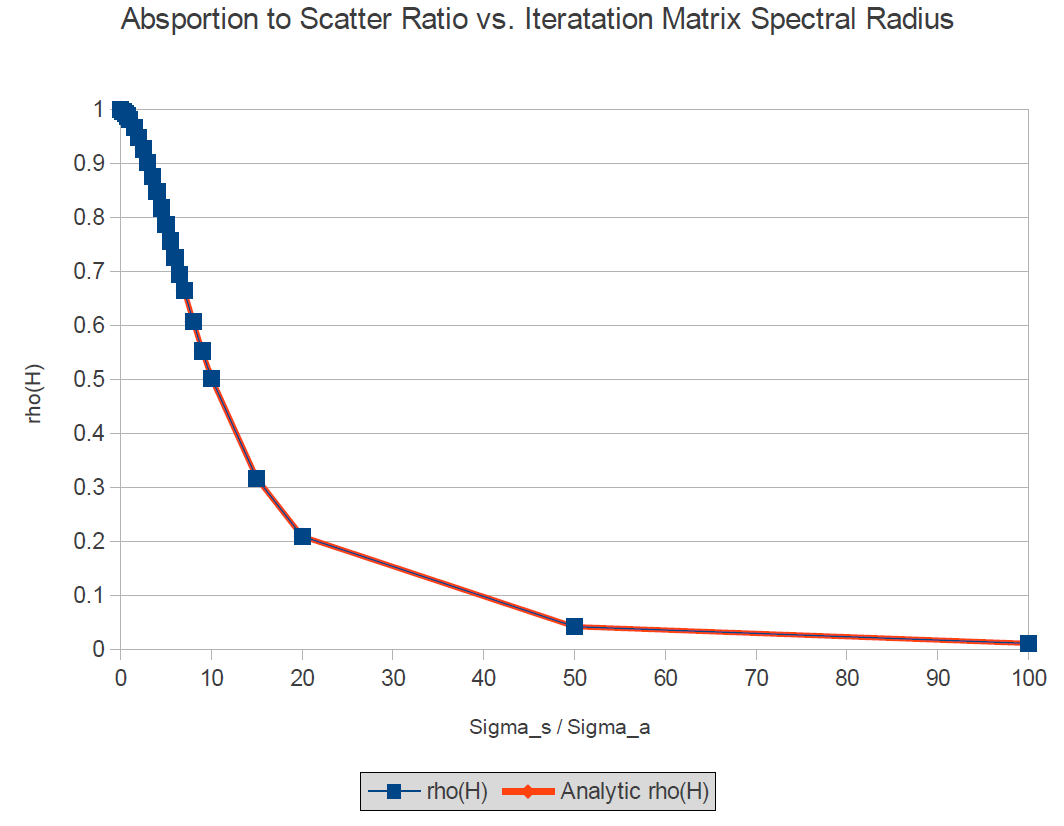
\includegraphics[width=4in,clip]{measured_spec_rad.png}
    \end{center}
    \caption{\textbf{Measured and analytic preconditioned diffusion
        operator spectral radius as a function of the absorption cross
        section to scattering cross section ratio.} \textit{Values of
        $h=0.01$, $h=0.1$, and $h=1.0$ were used. The red data was
        computed numerically by an Eigensolver while the black dashed
        data was generated by Eq~(\ref{eq:iteration_radius}).}}
    \label{fig:measured_spec_rad}
  \end{spacing}
\end{figure}

\subsection{Random Walk Length}
\label{subsec:walk_length}

With the spectral data in hand, we can go about setting up an
experiment to measure the length of the random walks generated by the
adjoint Neumann-Ulam solver. To do this, we again use a $100 \times
100$ square grid with $h=0.1$ and the absorption cross varied from 0
to 100 while the scattering cross section was fixed at unity. Three
weight cutoff values of \sn{1}{-2}, \sn{1}{-4}, and \sn{1}{-8} were
used with 10,000 histories generated by a point source source of
strength 1 in the center of the domain such that the boundary
conditions will have less of an effect on the length of the random
walks. For each of the histories, the number of transitions made was
tallied to provide an effective value of $k$ for each history. This
value was then averaged over all histories to get a measured value of
$k$ for the particular operator. On the left,
figure~\ref{fig:measured_length} these measurements as well as the
analytic result computed by Eq~(\ref{eq:analytic_k}) as a function of
the iteration matrix spectral radius, $\rho(\ve{H})$. On the right,
figure~\ref{fig:measured_length} gives the relative error between the
predicted and observed results. We note good qualitative agreement
between the measured and analytic results. However, we observe a
larger relative error for both long and short random walks.
\begin{figure}[ht!]
  \begin{spacing}{1.0}
    \begin{center}
      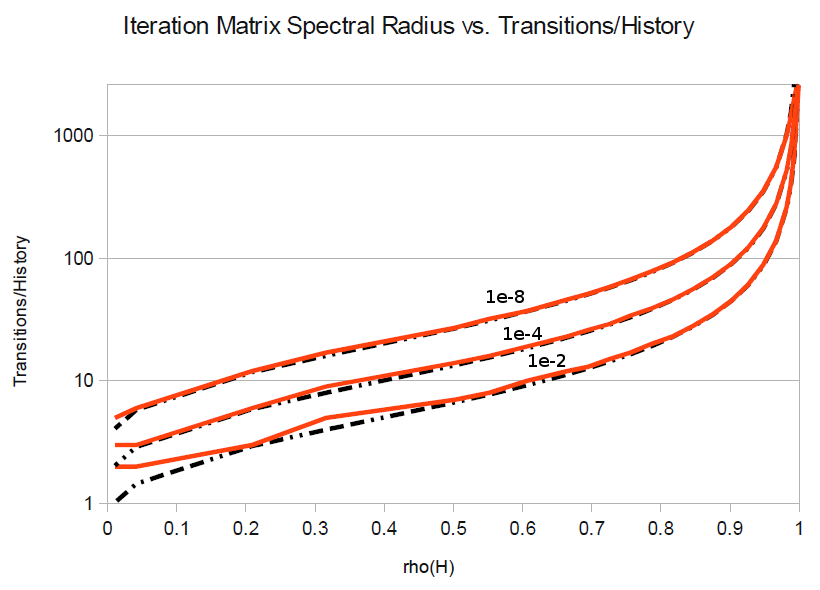
\includegraphics[width=6.5in,clip]{measured_length.png}
    \end{center}
    \caption{\textbf{Measured and analytic random walk length as a
        function of the iteration matrix spectral radius.} \textit{The
        weight cutoff was varied with \sn{1}{-2}, \sn{1}{-4}, and
        \sn{1}{-8}. In the left plot, the red data was computed
        numerically by an adjoint Neumann-Ulam implementation while
        the black dashed data was generated by
        Eq~(\ref{eq:analytic_k}). In the right plot, the relative
        error between the predicted and measured results is
        presented.}}
    \label{fig:measured_length}
  \end{spacing}
\end{figure}

\subsection{Domain Leakage}
\label{subsec:domain_leakage}

Finally, we seek to measure the leakage from a domain in a domain
decomposed Monte Carlo calculation and assess the quality of our
analytic relation for the optical thickness of domain and the
associated leakage approximations. For this experiment, a square grid
with $h=0.1$ was decomposed into 9 square domains, 3 in each cardinal
direction with measurements occurring in the central domain without
boundary grid points. For the cross sections, the absorption cross was
varied from 1 to 100 while the scattering cross section was set to
zero to create a purely absorbing environment. The optical thickness
of these domains will vary as a function of the absorption cross
section if the other parameters are fixed. To compute the optical
thickness, along with the spectral radius as given by
Eq~(\ref{eq:iteration_radius}), we also need the parameters $n_i$ and
$n_s$ which respectively describe the typical domain length and the
average number of states moved along that typical length per history
transition. For our grid above, the domains are varied in size with
$50 \times 50$, $100 \times 100$, and $200 \times 200$ cells giving
$n_i=50$, $n_i=100$, and $n_i=200$ grid points or states along the
typical length of the domain respectively with weight cutoff of
\sn{1}{-4}. Looking at the Laplacian stencil in
Eq~(\ref{eq:nine_point_stencil}), we see that all history transitions
will only move a single state in either the $i$ or $j$ directions due
to the symmetry of the problem. Furthermore, if we choose the $i$
direction, not all states we will transition to will move the history
in that direction. Therefore, we look to the definition of the
iteration matrix in Eq~(\ref{eq:iteration_stencil}) and the definition
of the adjoint probability matrix in Eq~(\ref{eq:adjoint_probability})
to estimate the $n_s$ parameter. For a particular transition starting
at state $(i,j)$, 6 of the 8 possible new states in the stencil move
the history in $i$ direction with relative coefficients of 4 for
moving in the $(\pm i,0)$ direction and of 1 for moving in the $(\pm
i,\pm j)$. These coefficients dictate the frequency those states are
visited relative to the others. For those 6 states we can visit along
the typical length, their sum is 12 out of the total 20 for the
coefficients for all possible states with their ratio giving $n_i =
\frac{3}{5}$.

To compute the leakage fraction numerically, \sn{3}{5} histories were
sampled from a uniform source of strength unity over the global
domain. At the start of a stage of histories, the number of histories
starting in the center domain was computed and as the stage
progressed, the number of histories that exited that domain was
tallied with the ratio of the two numbers providing a numerical
measure for the leakage fraction. Figure~\ref{fig:measured_leakage}
gives the domain leakage measurements for the domain in the center of
the global grid as well as the analytic result computed by
Eqs~(\ref{eq:wigner_domain_leakage}) and
(\ref{eq:mean_chord_domain_leakage}) as a function of the iteration
matrix spectral radius.
\begin{figure}[ht!]
  \begin{spacing}{1.0}
    \begin{center}
      \includegraphics[width=4.5in,clip]{leakage_variation.png}
    \end{center}
    \caption{\textbf{Measured and analytic domain leakage as a
        function of the iteration matrix spectral radius.} \textit{To
        test the behavior with respect to domain size, $n_i=50$,
        $n_i=100$,and $n_i=200$ were used. The red data was computed
        numerically by a domain-decomposed adjoint Neumann-Ulam
        implementation, the black dashed data was generated by
        Eq~(\ref{eq:mean_chord_domain_leakage}) using the mean-chord
        approximation, and the dashed-dotted black data was generated
        by Eq~(\ref{eq:wigner_domain_leakage}) using the Wigner
        rational approximation.}}
    \label{fig:measured_leakage}
  \end{spacing}
\end{figure}
Again, we note good qualitative agreement between the measured and
analytic quantities but we begin to see the limits of the leakage
approximations. To compare the quality of the two approximations, the
absolute error between the computed leakage fraction and that
generated by the Wigner rational and mean chord approximations is
plotted in Figure~\ref{fig:leakage_error} for all domain sizes
tested. 
\begin{figure}[ht!]
  \begin{spacing}{1.0}
    \begin{center}
      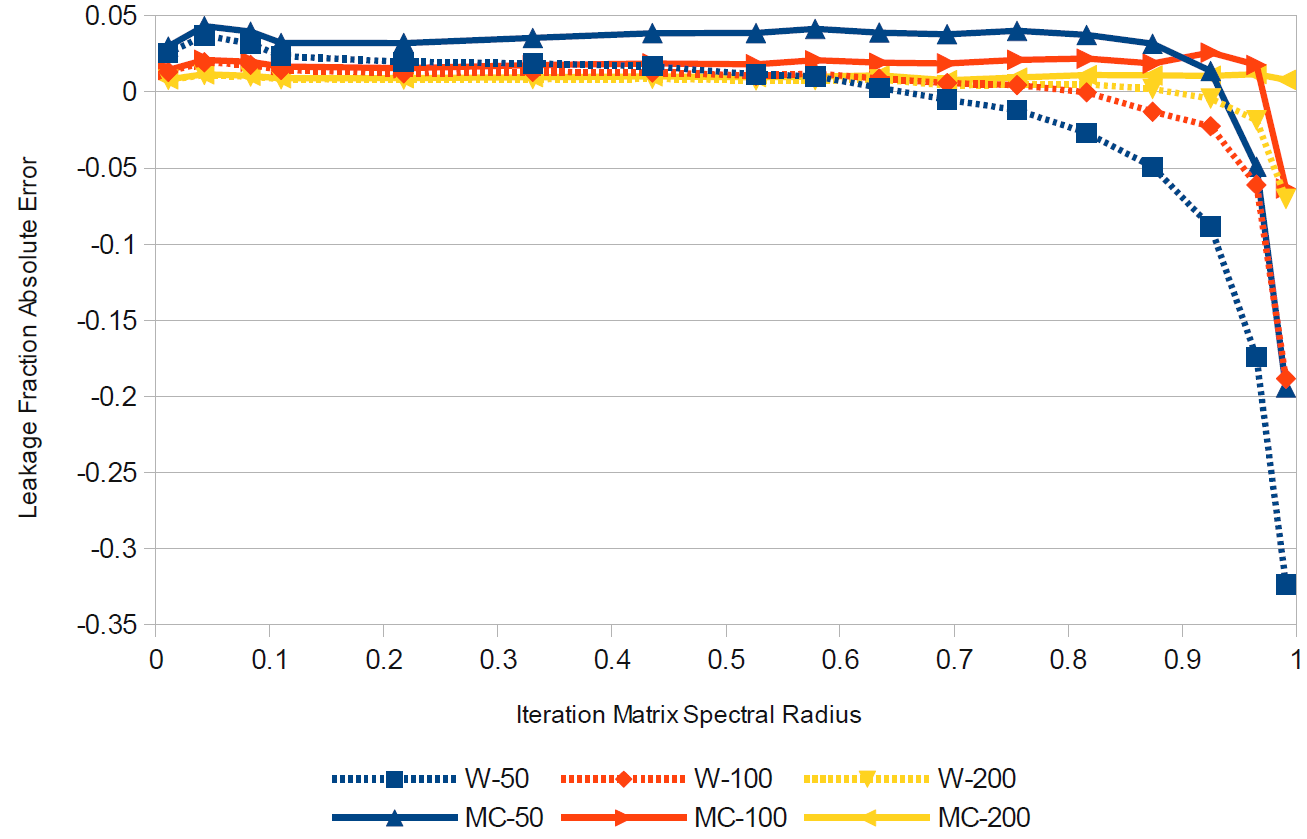
\includegraphics[width=4.5in,clip]{leakage_error.png}
    \end{center}
    \caption{\textbf{Measured and analytic domain leakage absolute error
        as a function of the iteration matrix spectral radius.}
      \textit{To test the behavior with respect to domain size, $n_i=50$
        (green), $n_i=100$ (blue), and $n_i=200$ (red) were used. The
        dashed lines represent the error using the Wigner rational
        approximation while the solid lines represent the error using
        the mean-chord approximation.}}
    \label{fig:leakage_error}
  \end{spacing}
\end{figure}
From these error results, the mean chord approximation is shown to
have a lower error for ill-conditioned systems as compared to the
Wigner approximation while the Wigner approximation produces less
error for more well-conditioned systems. We also note that for the
optically thick domains, the error is likely corresponded to that
observed in Figure~\ref{fig:measured_length} for the $k$ parameter
while the large relative error in $k$ for optically thin domains does
not affect the approximation significantly. In general, the mean chord
approximation is a better choice to estimate the leakage fraction in a
domain from the adjoint Neumann-Ulam method and except for a single
data point with $n_i=50$, the mean chord approximation yielded leakage
fractions within 0.05 of the measured results. As the domain becomes
more optically thick (with both increasing $n_i$ and decreasing
$\rho(\ve{H})$), the approximations are more accurate.

%%---------------------------------------------------------------------------%%
\section{CONCLUSIONS}

We have presented an analytic analysis of the domain decomposed
behavior of the adjoint Neumann Ulam method for linear operator
equations. Good agreement was observed between the derived analytic
relationships and numerical results generated by a domain decomposed
implementation of the adjoint method. 

In future work, these relationships will serve as guidelines for
selecting an appropriate parallel algorithm strategy and provide a
basis for performance models for future parallel implementations of
the adjoint Neumann-Ulam method. To be applicable to a broader range
of problems, these models could potentially be extended to
non-symmetric systems. In addition, these relations will be used to
analyze parallel implementations of Monte Carlo synthetic acceleration
methods that leverage the adjoint method and serve as an initial
grounds for assessing their feasibility for large-scale problems.

%%---------------------------------------------------------------------------%%
\section*{ACKNOWLEDGMENTS}

This work was performed under appointment to the Nuclear Regulatory
Commission Fellowship program at the University of Wisconsin - Madison
Engineering Physics Department.

%%---------------------------------------------------------------------------%%
%%\Section*{REFERENCES}
\setlength{\baselineskip}{12pt}
\bibliographystyle{ieeetr}
\bibliography{references}

\end{document}


